\documentclass[svgnames,dvipsnames,hyperref={bookmarks=false},usepdftitle=false]{beamer}
\usetheme{scaladays}
\usepackage{tikz}
\usetikzlibrary[arrows.meta]

\title{No, macros are not going away}
\author{Eugene Burmako (\href{https://twitter.com/xeno_by}{@xeno{\textunderscore}by})}
\institute{
\includegraphics[height=2cm]{epfl.png}}
\date{17 June 2016}
\hypersetup{pdfauthor={Eugene Burmako},pdftitle={Metaprogramming 2.0}}

\begin{document}

\titleframe

\begin{frame}{Today's talk}
\begin{itemize}
\item What is scala.meta?
\item What can scala.meta do?
\item Why should you care?
\item What will happen next?
\end{itemize}
\end{frame}

\begin{frame}{scala.meta is a dream}
\begin{center}

\includegraphics[height=6cm]{is-a-dream.png}
\end{center}
\end{frame}

\begin{frame}{scala.meta is an active project}
\vskip20pt
\begin{center}

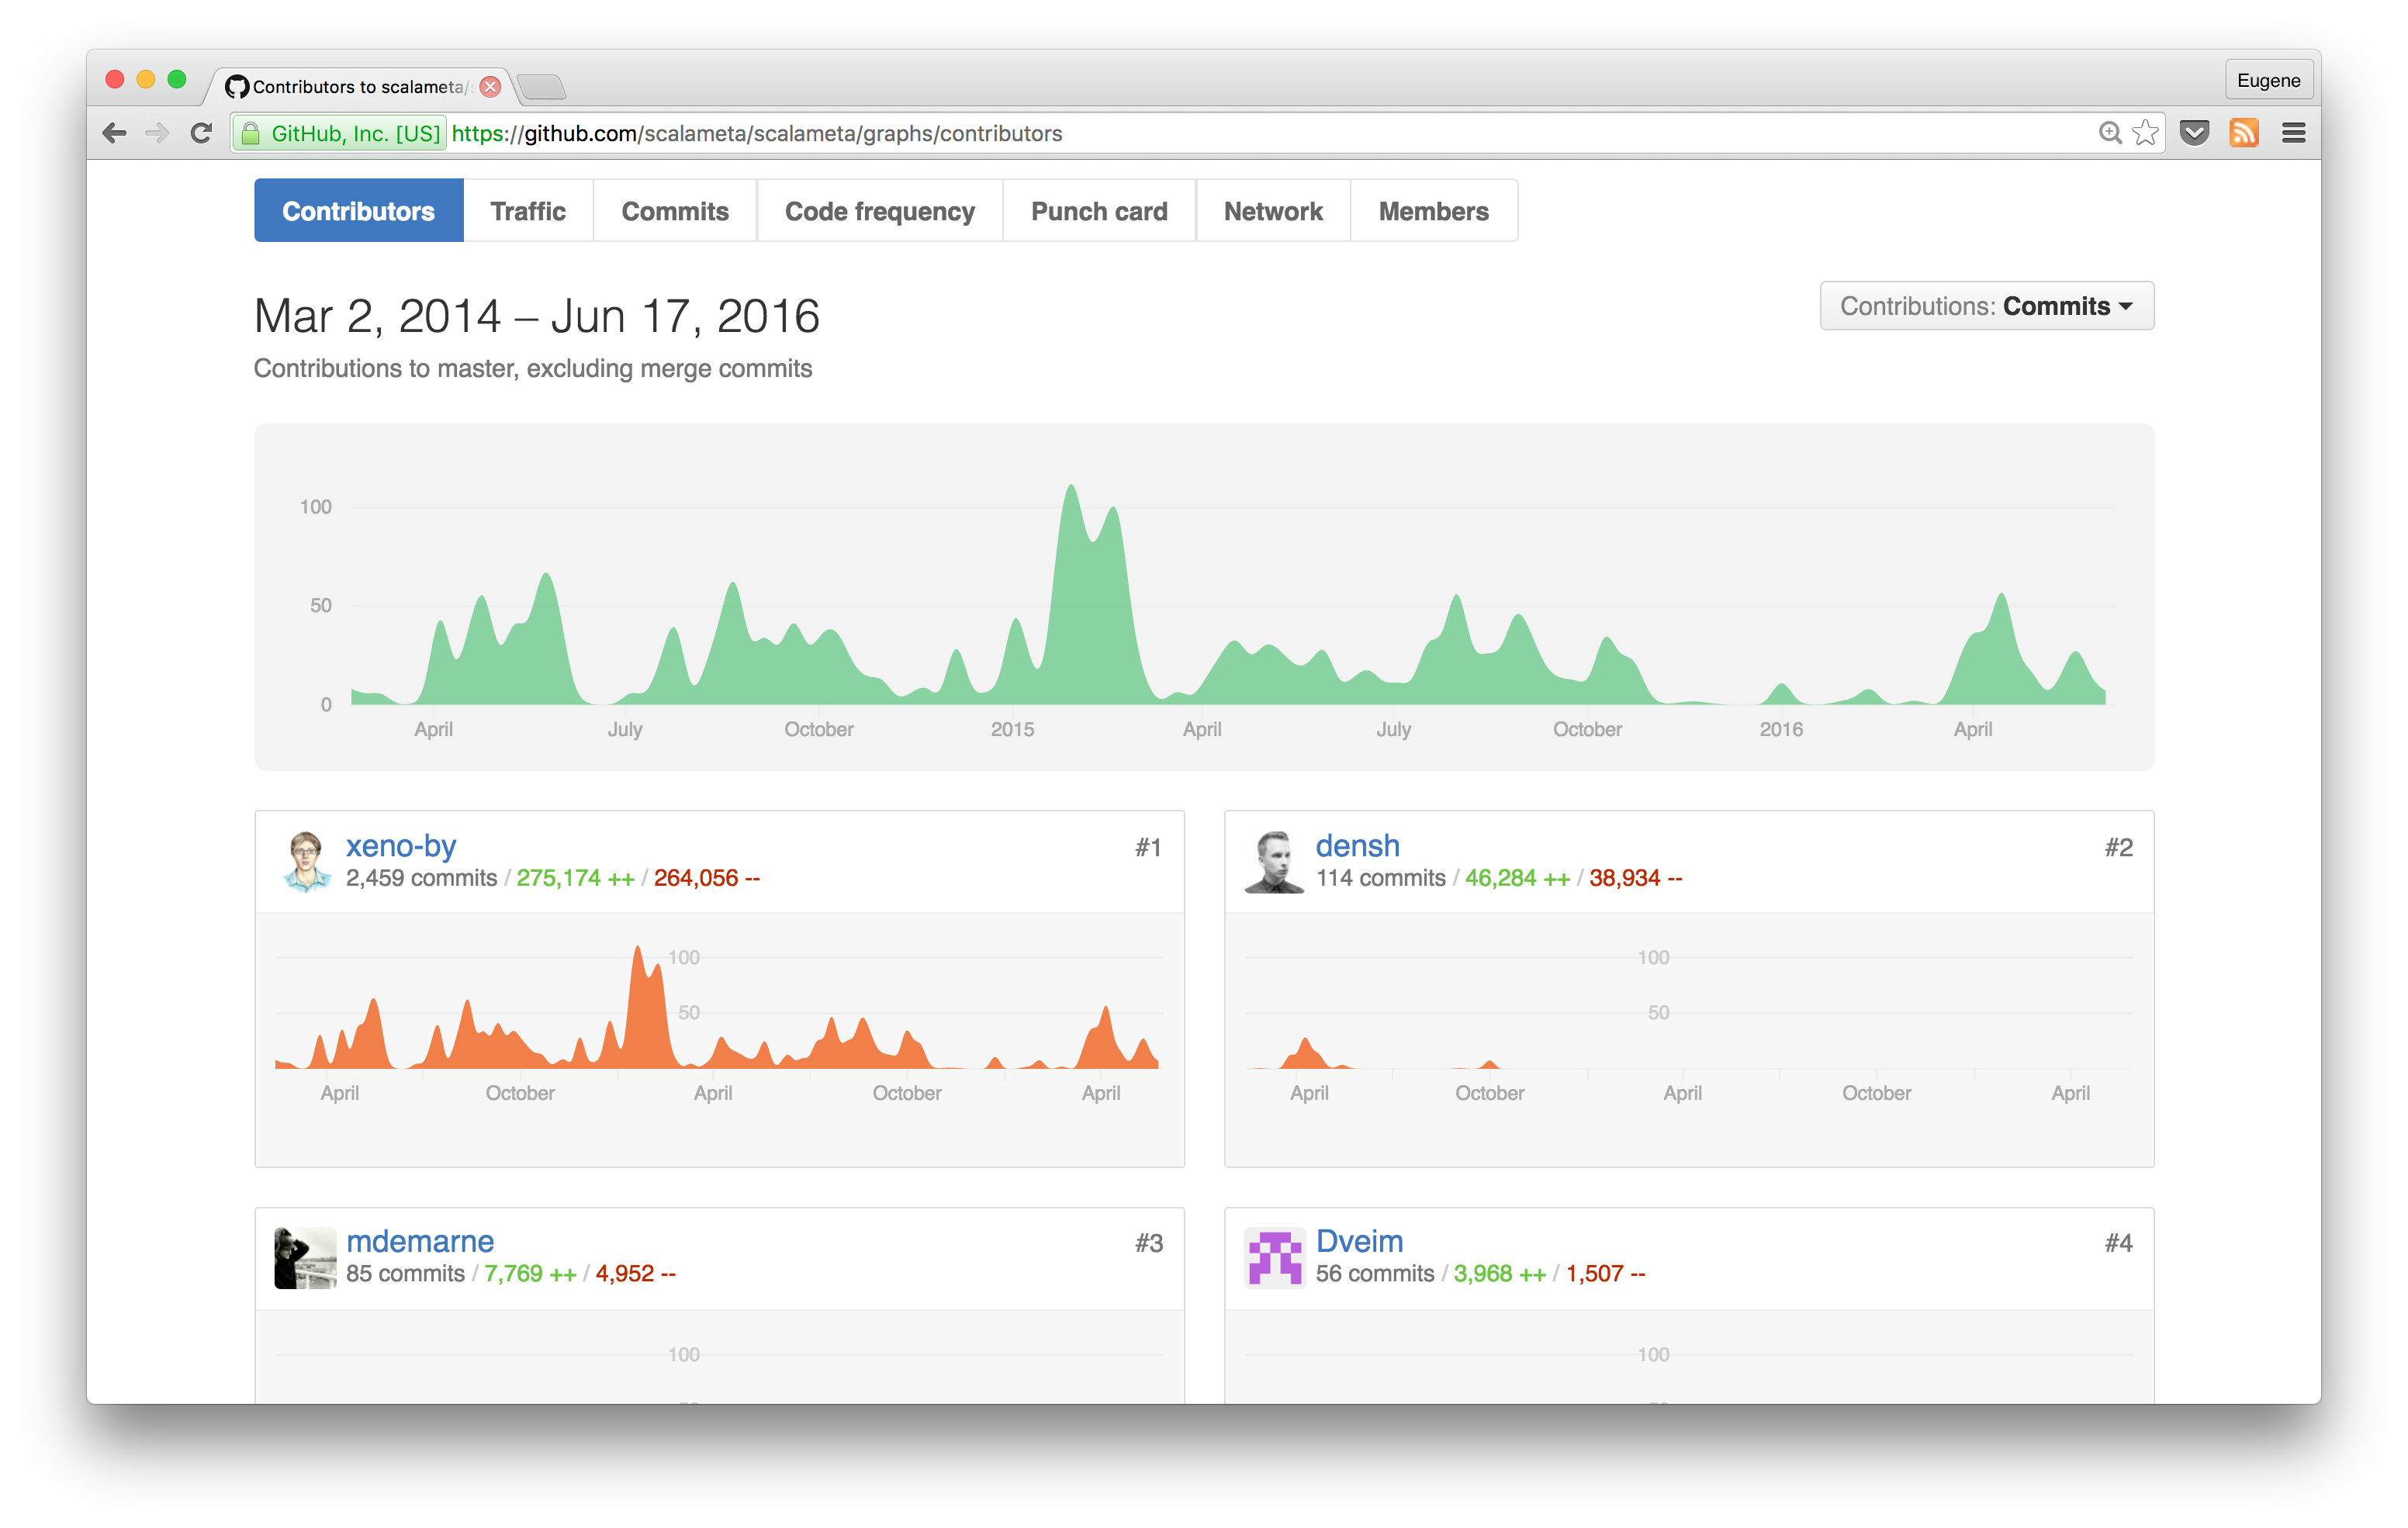
\includegraphics[height=7.5cm]{is-an-active-project.png}
\end{center}
\end{frame}

\begin{frame}{scala.meta is a community}
\vskip20pt
\begin{center}
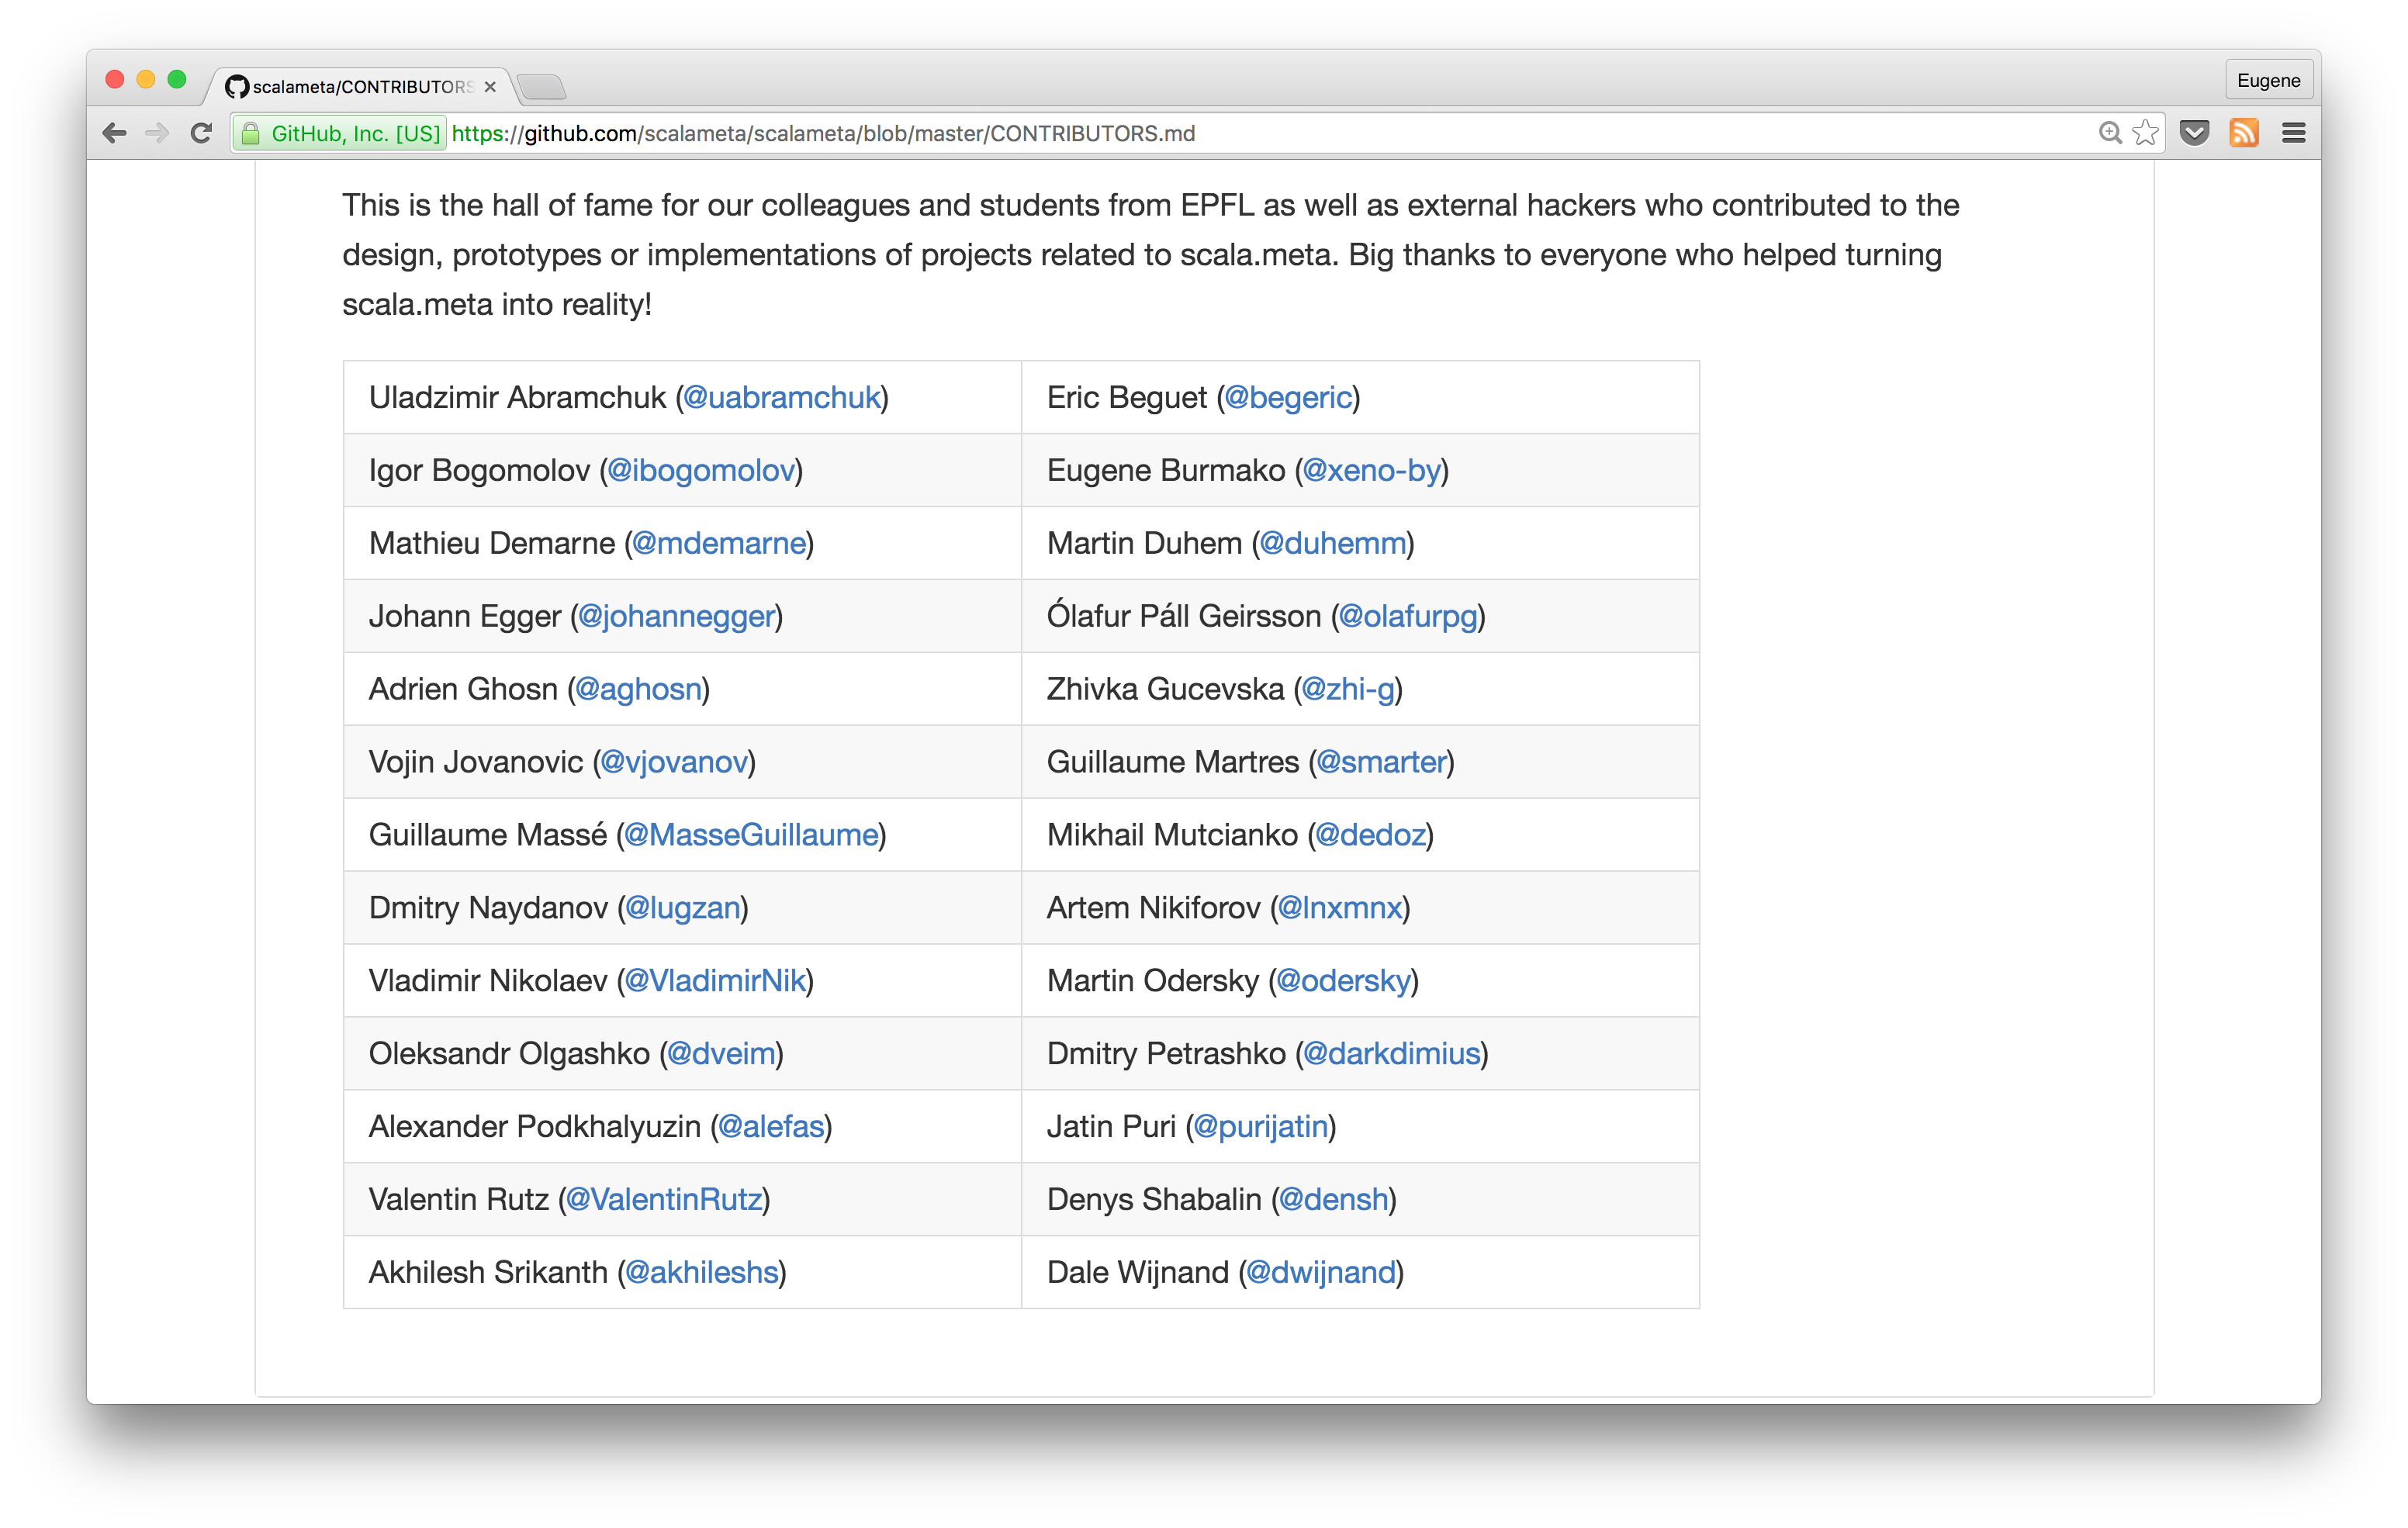
\includegraphics[height=7.5cm]{is-a-community.png}
\end{center}
\end{frame}

\begin{frame}{scala.meta is a product}
\vskip20pt
\begin{center}
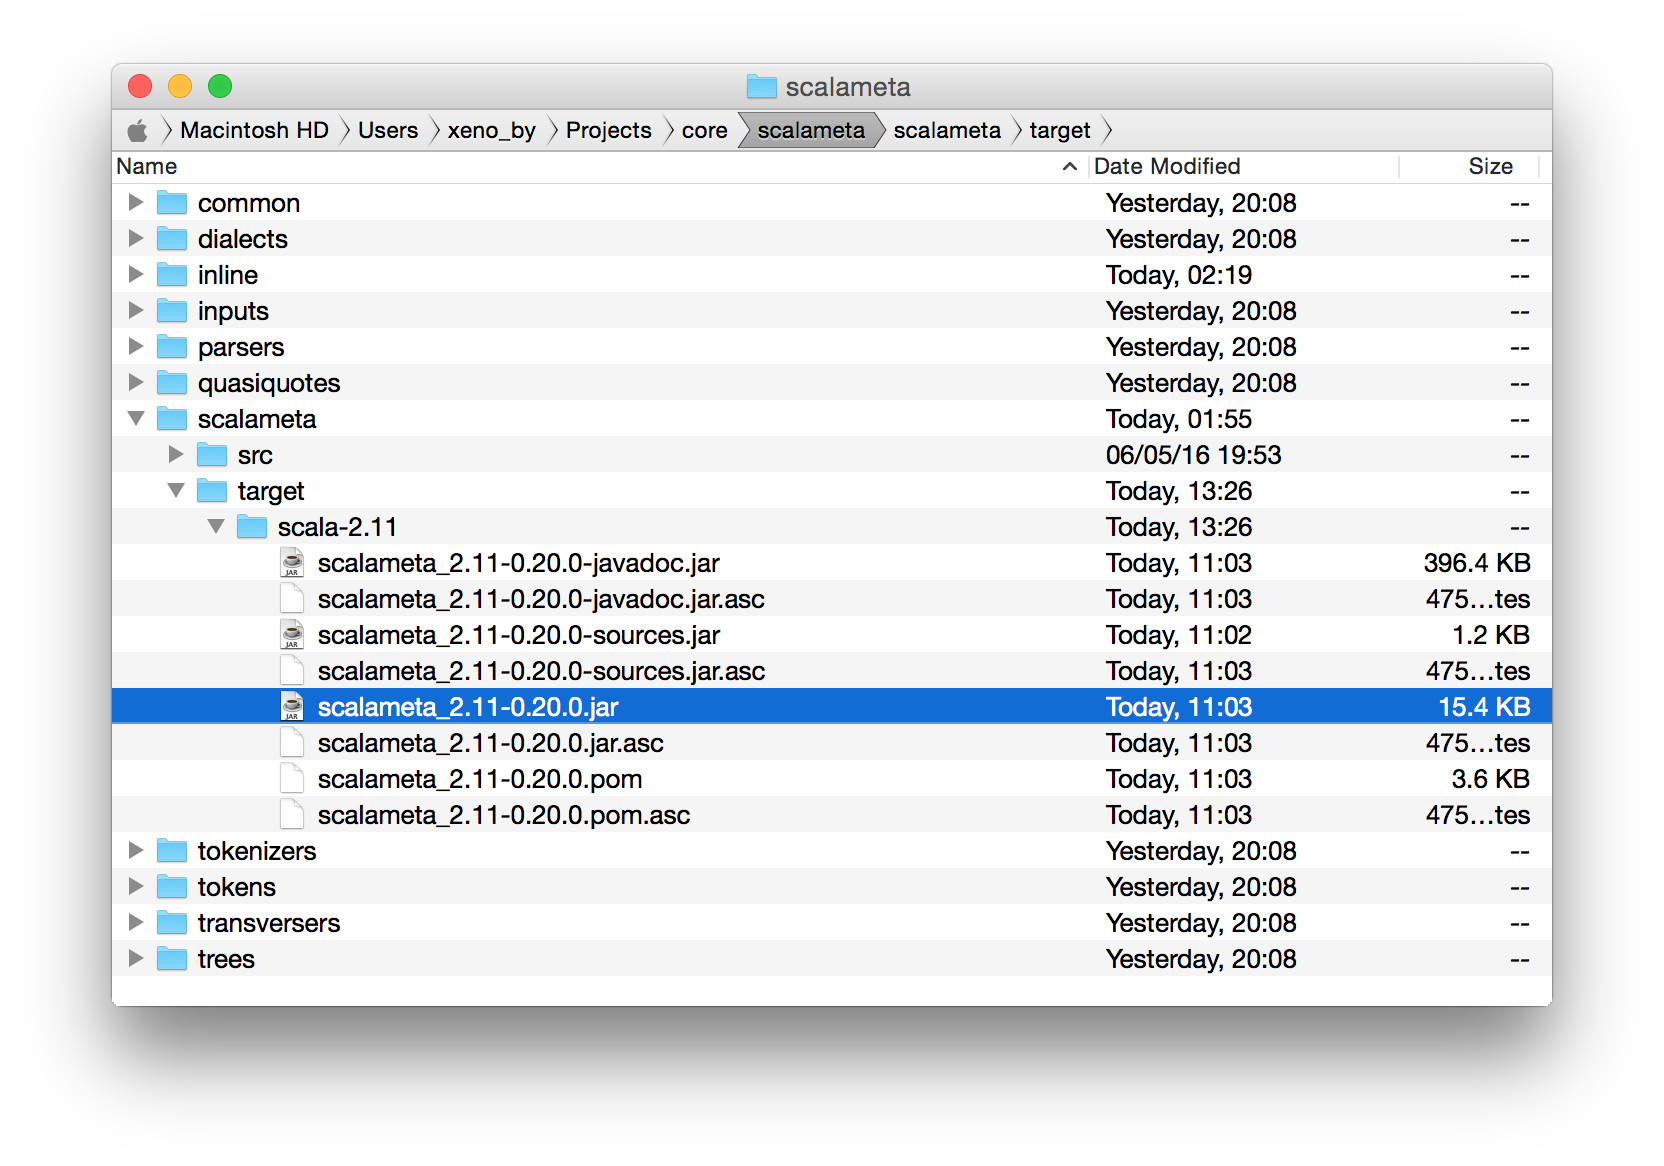
\includegraphics[height=8cm]{is-a-product.png}
\end{center}
\end{frame}

\begin{frame}{scala.meta is officially endorsed}
\vskip20pt
\begin{center}
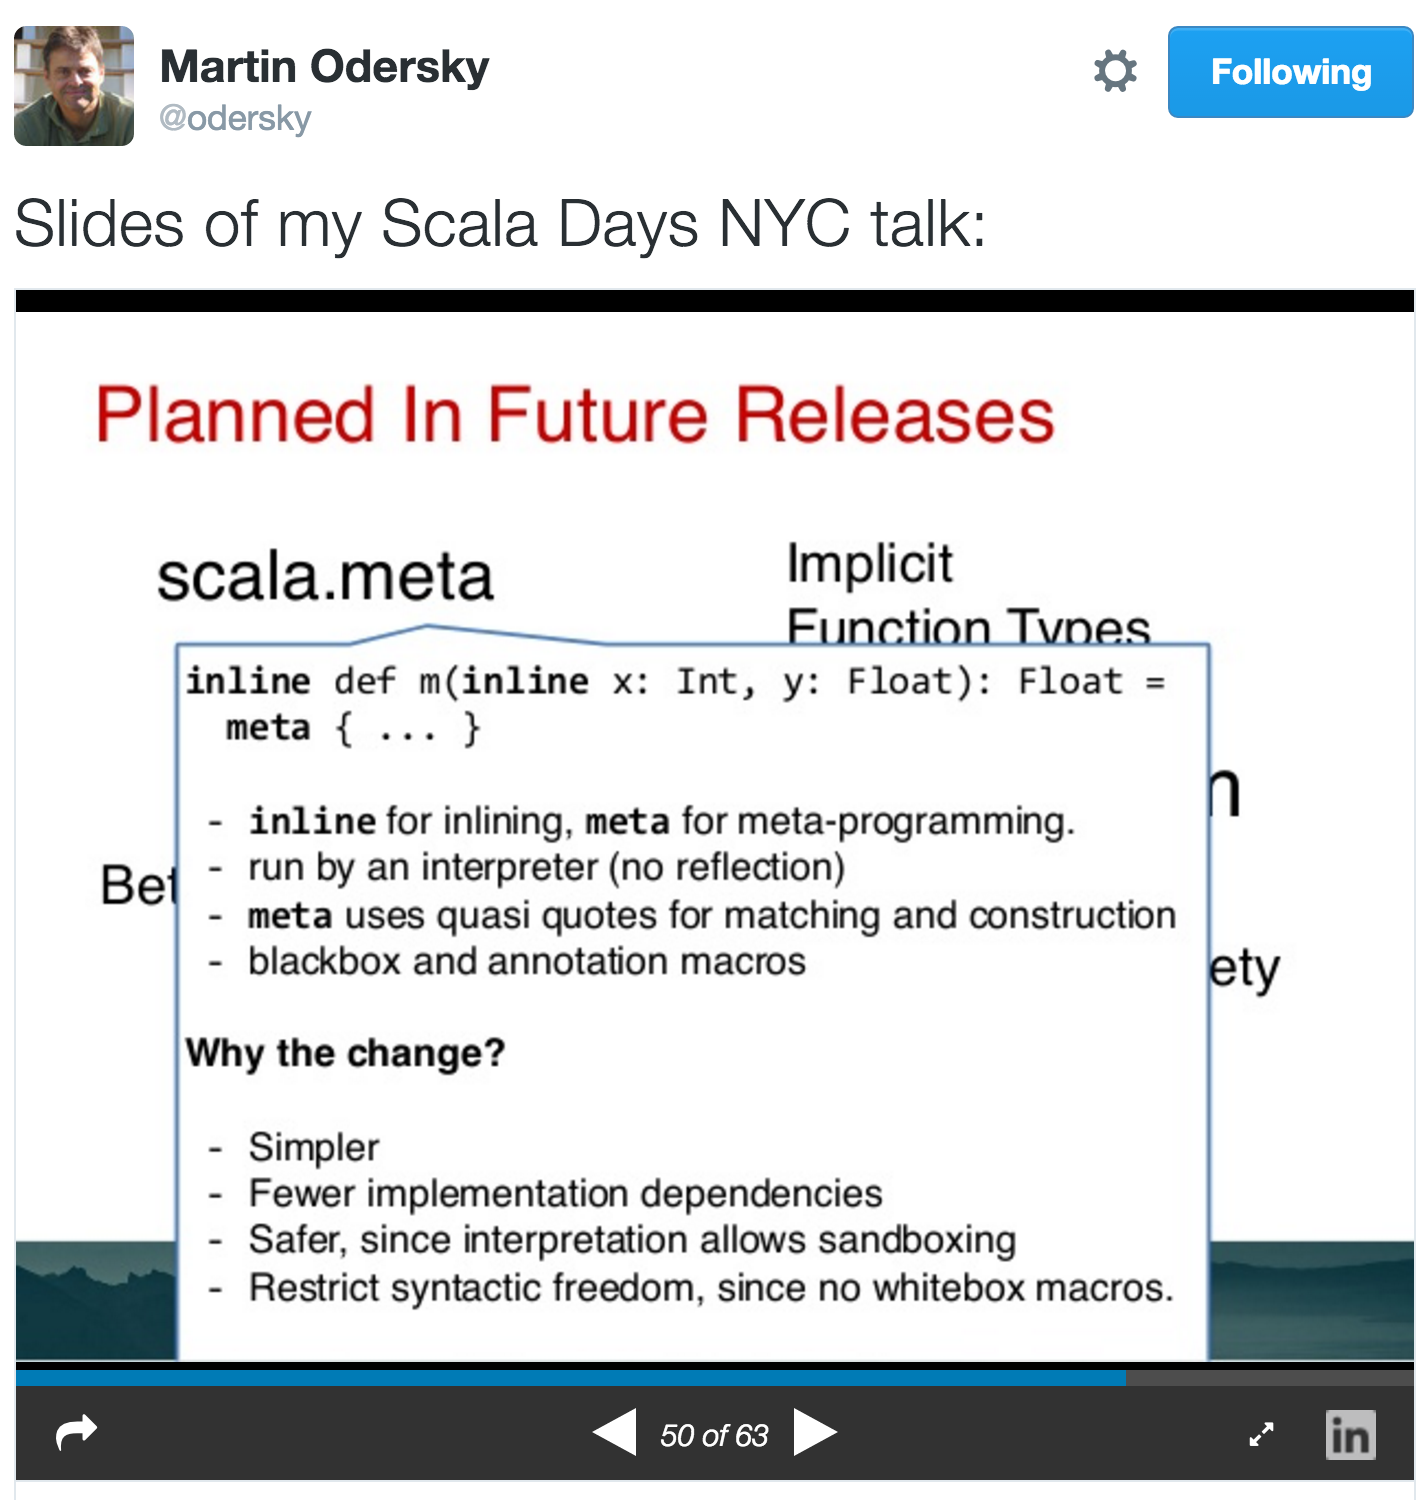
\includegraphics[height=7.5cm]{is-officially-endorsed.png}
\end{center}
\end{frame}

\sectionframe{Part 1: What can scala.meta do?}

\begin{frame}{Project status}
\begin{itemize}
\item 17 Jun 2014: ``Easy metaprogramming for everyone!''
\item<2-> 17 Jun 2016: 3191 commits and 27 milestones later...
\item<3-> \alert<3->{We're finally releasing v1.0!}
\end{itemize}
\end{frame}

\begin{frame}{Supported functionality}
\begin{itemize}
\item Vendor-neutral tree interchange format
\item High-fidelity parsing
\item First-class tokens
\end{itemize}
\end{frame}

\begin{frame}[fragile]
\frametitle<1>{Parsing: easy to get started}
\frametitle<2>{Parsing: remember all syntactic details}
\begin{semiverbatim}
scala> import scala.meta._
import scala.meta._

scala> "x + y".parse[Term]
res0: scala.meta.parsers.Parsed[scala.meta.Term] = x + y

\only<2->{scala> "x + y // hello world".parse[Term]}
\only<2->{res1: scala.meta.parsers.Parsed[scala.meta.Term] = }
\only<2->{x + y // hello world}
\end{semiverbatim}
\end{frame}

\begin{frame}[fragile]{Tokens: remember all syntactic details}
\begin{semiverbatim}
scala> val add = "x + y // hello world".parse[Term].get
add: scala.meta.Term = x + y // hello world

\only<1->{scala> add.tokens}
\only<1->{res2: scala.meta.tokens.Tokens =}
\only<1->{Tokens(, x,  , +,  , y,  , // hello world, )}

\only<2->{scala> add.tokens.structure}
\only<2->{res3: String = Tokens(BOF [0..0), x [0..1),  [1..2), }
\only<2->{+ [2..3), [3..4), y [4..5),   [5..6), }
\only<2->{// hello world [6..20), EOF [20..20))}
\end{semiverbatim}
\end{frame}

\begin{frame}[fragile]{Parsing: support for dialects}
\begin{semiverbatim}
scala> val sbtBuild = new File(".../project/plugins.sbt")
sbtBuild: java.io.File = .../project/plugins.sbt

\only<2->{scala> \alert{scala.meta.dialects.Sbt0136}(sbtBuild).parse[Source]}
\only<2->{res4: scala.meta.parsers.Parsed[scala.meta.Source] =}
\only<2->{}
\only<2->{addSbtPlugin("com.typesafe.sbt" \% "sbt-pgp" \% "0.8.1")}
\only<2->{}
\only<2->{addSbtPlugin("com.eed3si9n" \% "sbt-assembly" \% "0.11.2")}
\only<2->{...}
\end{semiverbatim}
\end{frame}

\begin{frame}[fragile]
\frametitle<1>{Quasiquotes: stealing better parts of scala.reflect}
\begin{semiverbatim}
scala> q"x + y"
res5: scala.meta.Term.ApplyInfix = x + y

scala> val q"\$a + \$b" = res5
a: scala.meta.Term = x
b: scala.meta.Term.Arg = y
\end{semiverbatim}
\end{frame}

\sectionframe{Part 2: Why should you care?}

\begin{frame}{Why should you care?}
Scala.meta provides unique features that enable much better tools
\end{frame}

\sectionframe{Case study: Macros}

\begin{frame}{Macros are dead?}
\vskip20pt
\begin{center}
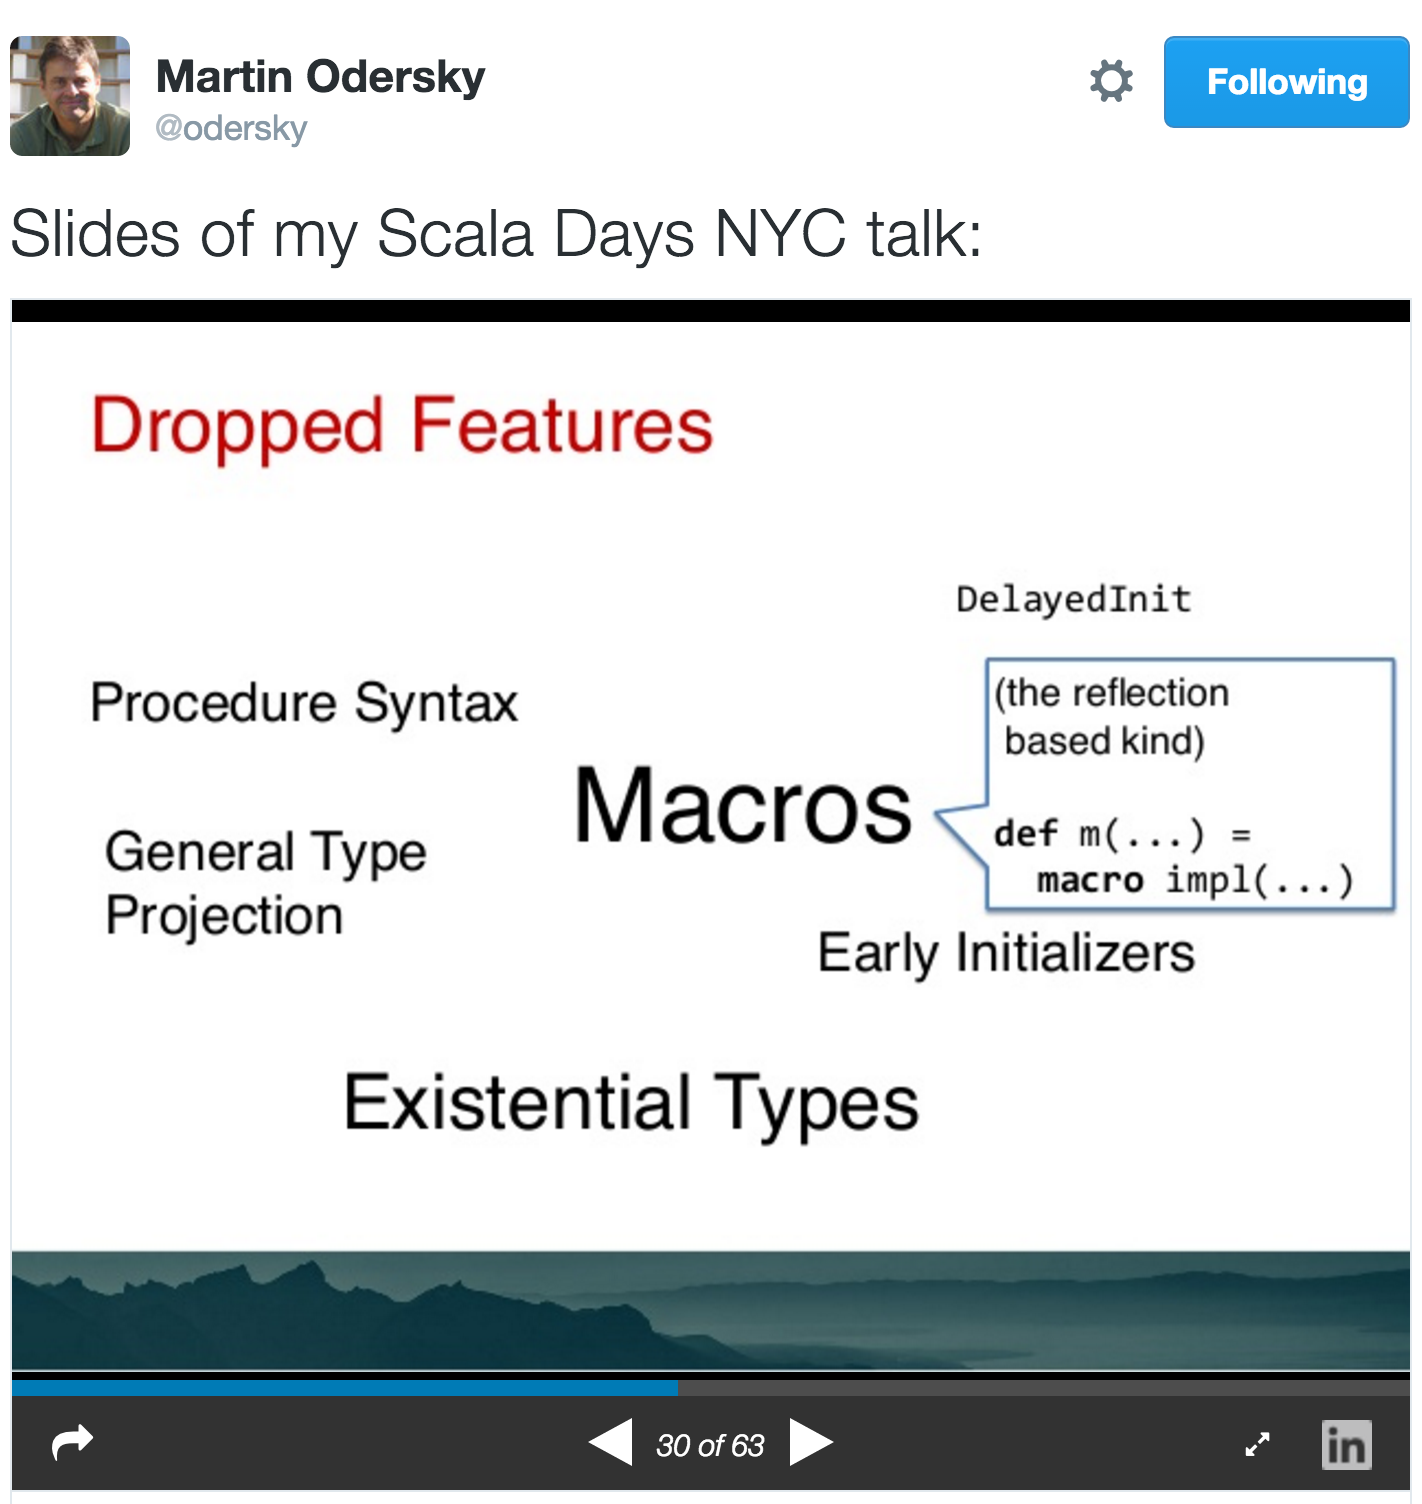
\includegraphics[height=7.5cm]{macros-are-dead.png}
\end{center}
\end{frame}

\begin{frame}{Macros are bad}
\begin{itemize}
\item Hard to write
\item Don't work with tools well
\end{itemize}
\end{frame}

\begin{frame}[fragile]{Example: the @main macro}
\begin{semiverbatim}
@main object Test \{
  println("hello world")
\}

                          \arrowdown

object Test \{
  def main(args: Array[String]): Unit = \{
    println("hello world")
  \}
\}
\end{semiverbatim}
\end{frame}

\begin{frame}[fragile]
\frametitle<1,2>{Example: the @main macro}
\frametitle<3->{Really hard to write!}
\begin{semiverbatim}
class main extends scala.annotation.StaticAnnotation \{
  \alert<3>{def macroTransform(annottees: Any*): Any =}
    \alert<3>{macro Macros.impl}
\}

\only<2->{\alert<3>{import scala.reflect.macros.whitebox.Context}}
\only<2->{\alert<3>{object Macros \{}}
\only<2->{\alert<3>{  def impl(c: Context)(annottees: c.Tree*): c.Tree = \{}}
\only<2->{\alert<3>{    import c.universe.\_}}
\only<2->{    val q"object \$name \{ ..\$stats \}" = annottees.head}
\only<2->{    val main = q"""}
\only<2->{      def main(args: Array[String]): Unit = \{ ..\$stats \}}
\only<2->{    """}
\only<2->{    q"object \$name \{ \$main \}"}
\only<2->{\alert<3>{  \}}}
\only<2->{\alert<3>{\}}}
\end{semiverbatim}
\end{frame}

\begin{frame}{Don't work with tools well}
\begin{itemize}
\item If we make a typo in macro code, IDEs won't help us
\item If we change macro code, SBT isn't going to recompile
\end{itemize}
\end{frame}

\begin{frame}{On the other hand, macros are great}
\begin{itemize}
\item Enable unique functionality
\item Frequently used by library authors
\item We can't really do without them!
\end{itemize}
\end{frame}

\begin{frame}{The new future for macros}
\begin{itemize}
\item We thought real hard how to make macros better
\item We found that most of the complexity is incidental
\item This is how \texttt{scala.meta} was conceived two years ago
\item Now that v1.0 is here, it's time to unveil our plans
\end{itemize}
\end{frame}

{
  \setbeamertemplate{footline}{}
  \setbeamercolor{background canvas}{bg=black}
  \begin{frame}{}
  \vskip20pt
  \begin{center}
  
\includegraphics[height=7.6cm]{return-of-the-king.png}
  \end{center}
  \end{frame}
}

\begin{frame}{The new future for macros}
\begin{itemize}
\item We got to the essence of macros and found two orthogonal concepts
\item \texttt{inline} for inlining and \texttt{meta} for metaprogramming
\item For details: \text{\color{blue}\href{https://github.com/scalameta/sips/blob/master/sips/drafts/sip-inlinemeta.md}{SIP NN: Inline Definitions and Meta Expressions}}
\end{itemize}
\end{frame}

\begin{frame}[fragile]{Example: the new @main macro}
\begin{semiverbatim}
import scala.meta._

class main extends scala.annotation.StaticAnnotation \{
  inline def apply(defn: Any) = meta \{
    val q"object \$name \{ ..\$stats \}" = defn
    val main = q"""
      def main(args: Array[String]): Unit = \{ ..\$stats \}
    """
    q"object \$name \{ \$main \}"
  \}
\}
\end{semiverbatim}
\end{frame}


\begin{frame}[fragile]{Example: the new @main macro}
\small{
\begin{semiverbatim}
@main object Test \{
  println("hello world")
\}

\only<2->{                          \arrowdown}
\only<2->{}
\only<2->{meta \{}
\only<2->{  val q"object \$name \{ ..\$stats \}" = \alert{q"object Test \{ ... \}"}}
\only<2->{  val main = q"def main(args: Array[String]): Unit = \{ ..\$stats \}"}
\only<2->{  q"object \$name \{ \$main \}"}
\only<2->{\}}

\only<3->{                          \arrowdown}
\only<3->{}
\only<3->{object Test \{}
\only<3->{  def main(args: Array[String]): Unit = \{}
\only<3->{    println("hello world")}
\only<3->{  \}}
\only<3->{\}}
\end{semiverbatim}}
\end{frame}

\begin{frame}{Macro support in IntelliJ IDEA}
\begin{itemize}
\item We've been collaborating since the early days of Scala macros
\item Some results are already available in production builds
\item Scala.meta provides a principled foundation for macro support
\end{itemize}
\end{frame}

\begin{frame}[c, fragile]{Live demo!}
\vskip20pt
\begin{center}
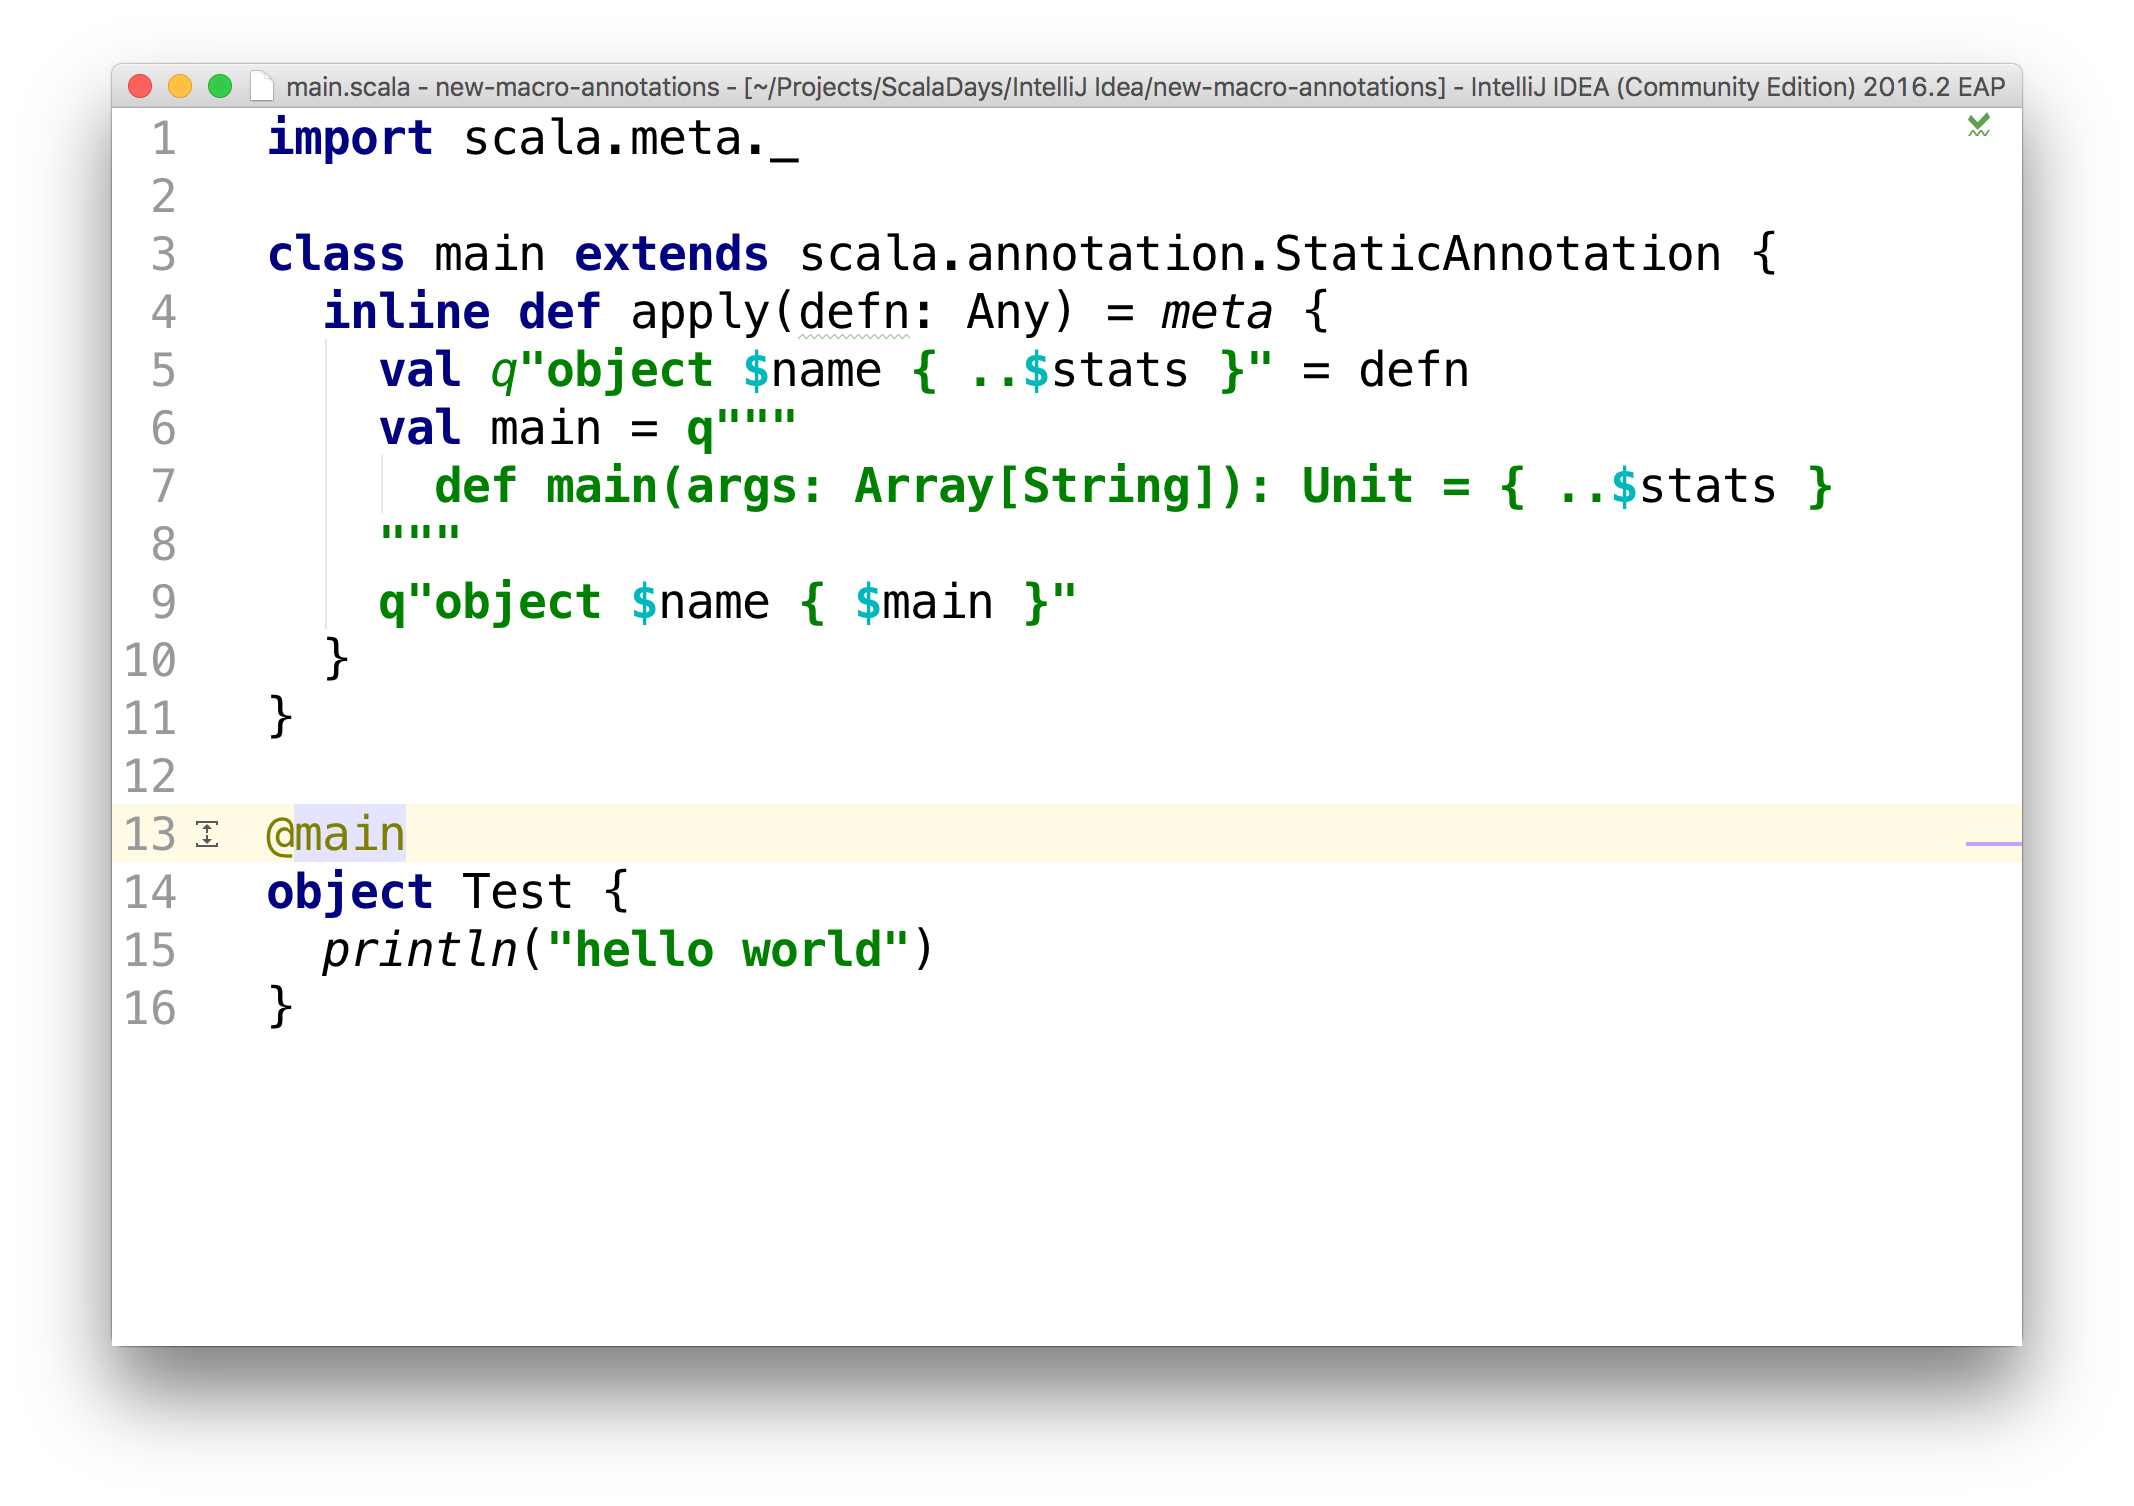
\includegraphics[width=12cm]{intellij.png}
\end{center}
\end{frame}

\begin{frame}{How IntelliJ macro support works}
\begin{itemize}
\item IntelliJ provides typechecking and name resolution
\item This information flows into scala.meta via an integration layer
\item Macro expansions are fed back into IntelliJ
\item Live feedback, precise error messages, and other goodies!
\end{itemize}
\end{frame}

\begin{frame}{Future plans for IntelliJ macro support}
\begin{itemize}
\item Live resolve of transformed trees
\item Looking forward to scala.meta's semantic API
\item Interpreting scala.meta programs
\end{itemize}
\end{frame}

\begin{frame}{Summary}
\begin{itemize}
\item Macros are not going away
\item Will be replaced with a better version based on scala.meta
\item Easier to write, better IDE support
\item We've got a prototype working, will be upgrading it in the near future
\end{itemize}
\end{frame}

\sectionframe{Case study: Dotty linker}

\begin{frame}{Dotty linker}
\begin{itemize}
\item Experimental whole program optimizer for Scala
\item Auto specialization
\item Recent addition: rewrite rules
\item Check out \text{\color{blue}{\href{https://d-d.me/talks/scaladays2016-linker}{Dmitry's talk}}} for details
\end{itemize}
\end{frame}

\begin{frame}[fragile]{Rewrite rules}
\begin{semiverbatim}
import dotty.linker._

@rewrites
object Rewrites \{
  def metaRule[T](x: ExistingClass) =
    Rewrite(from = x.existingSlowMethod(...),
              to = meta \{ /* entry point to scala.meta */ \})
\}
\end{semiverbatim}
\end{frame}

\sectionframe{Case study: Codacy}

\begin{frame}{Codacy}
\begin{itemize}
\item Codacy is a Portuguese startup doing static code analysis
\item Web application that connects to GitHub/Bitbucket projects
\item Supporting various languages including Scala via open-source tools
\end{itemize}
\end{frame}

\begin{frame}[c, fragile]{Live demo!}
\begin{center}
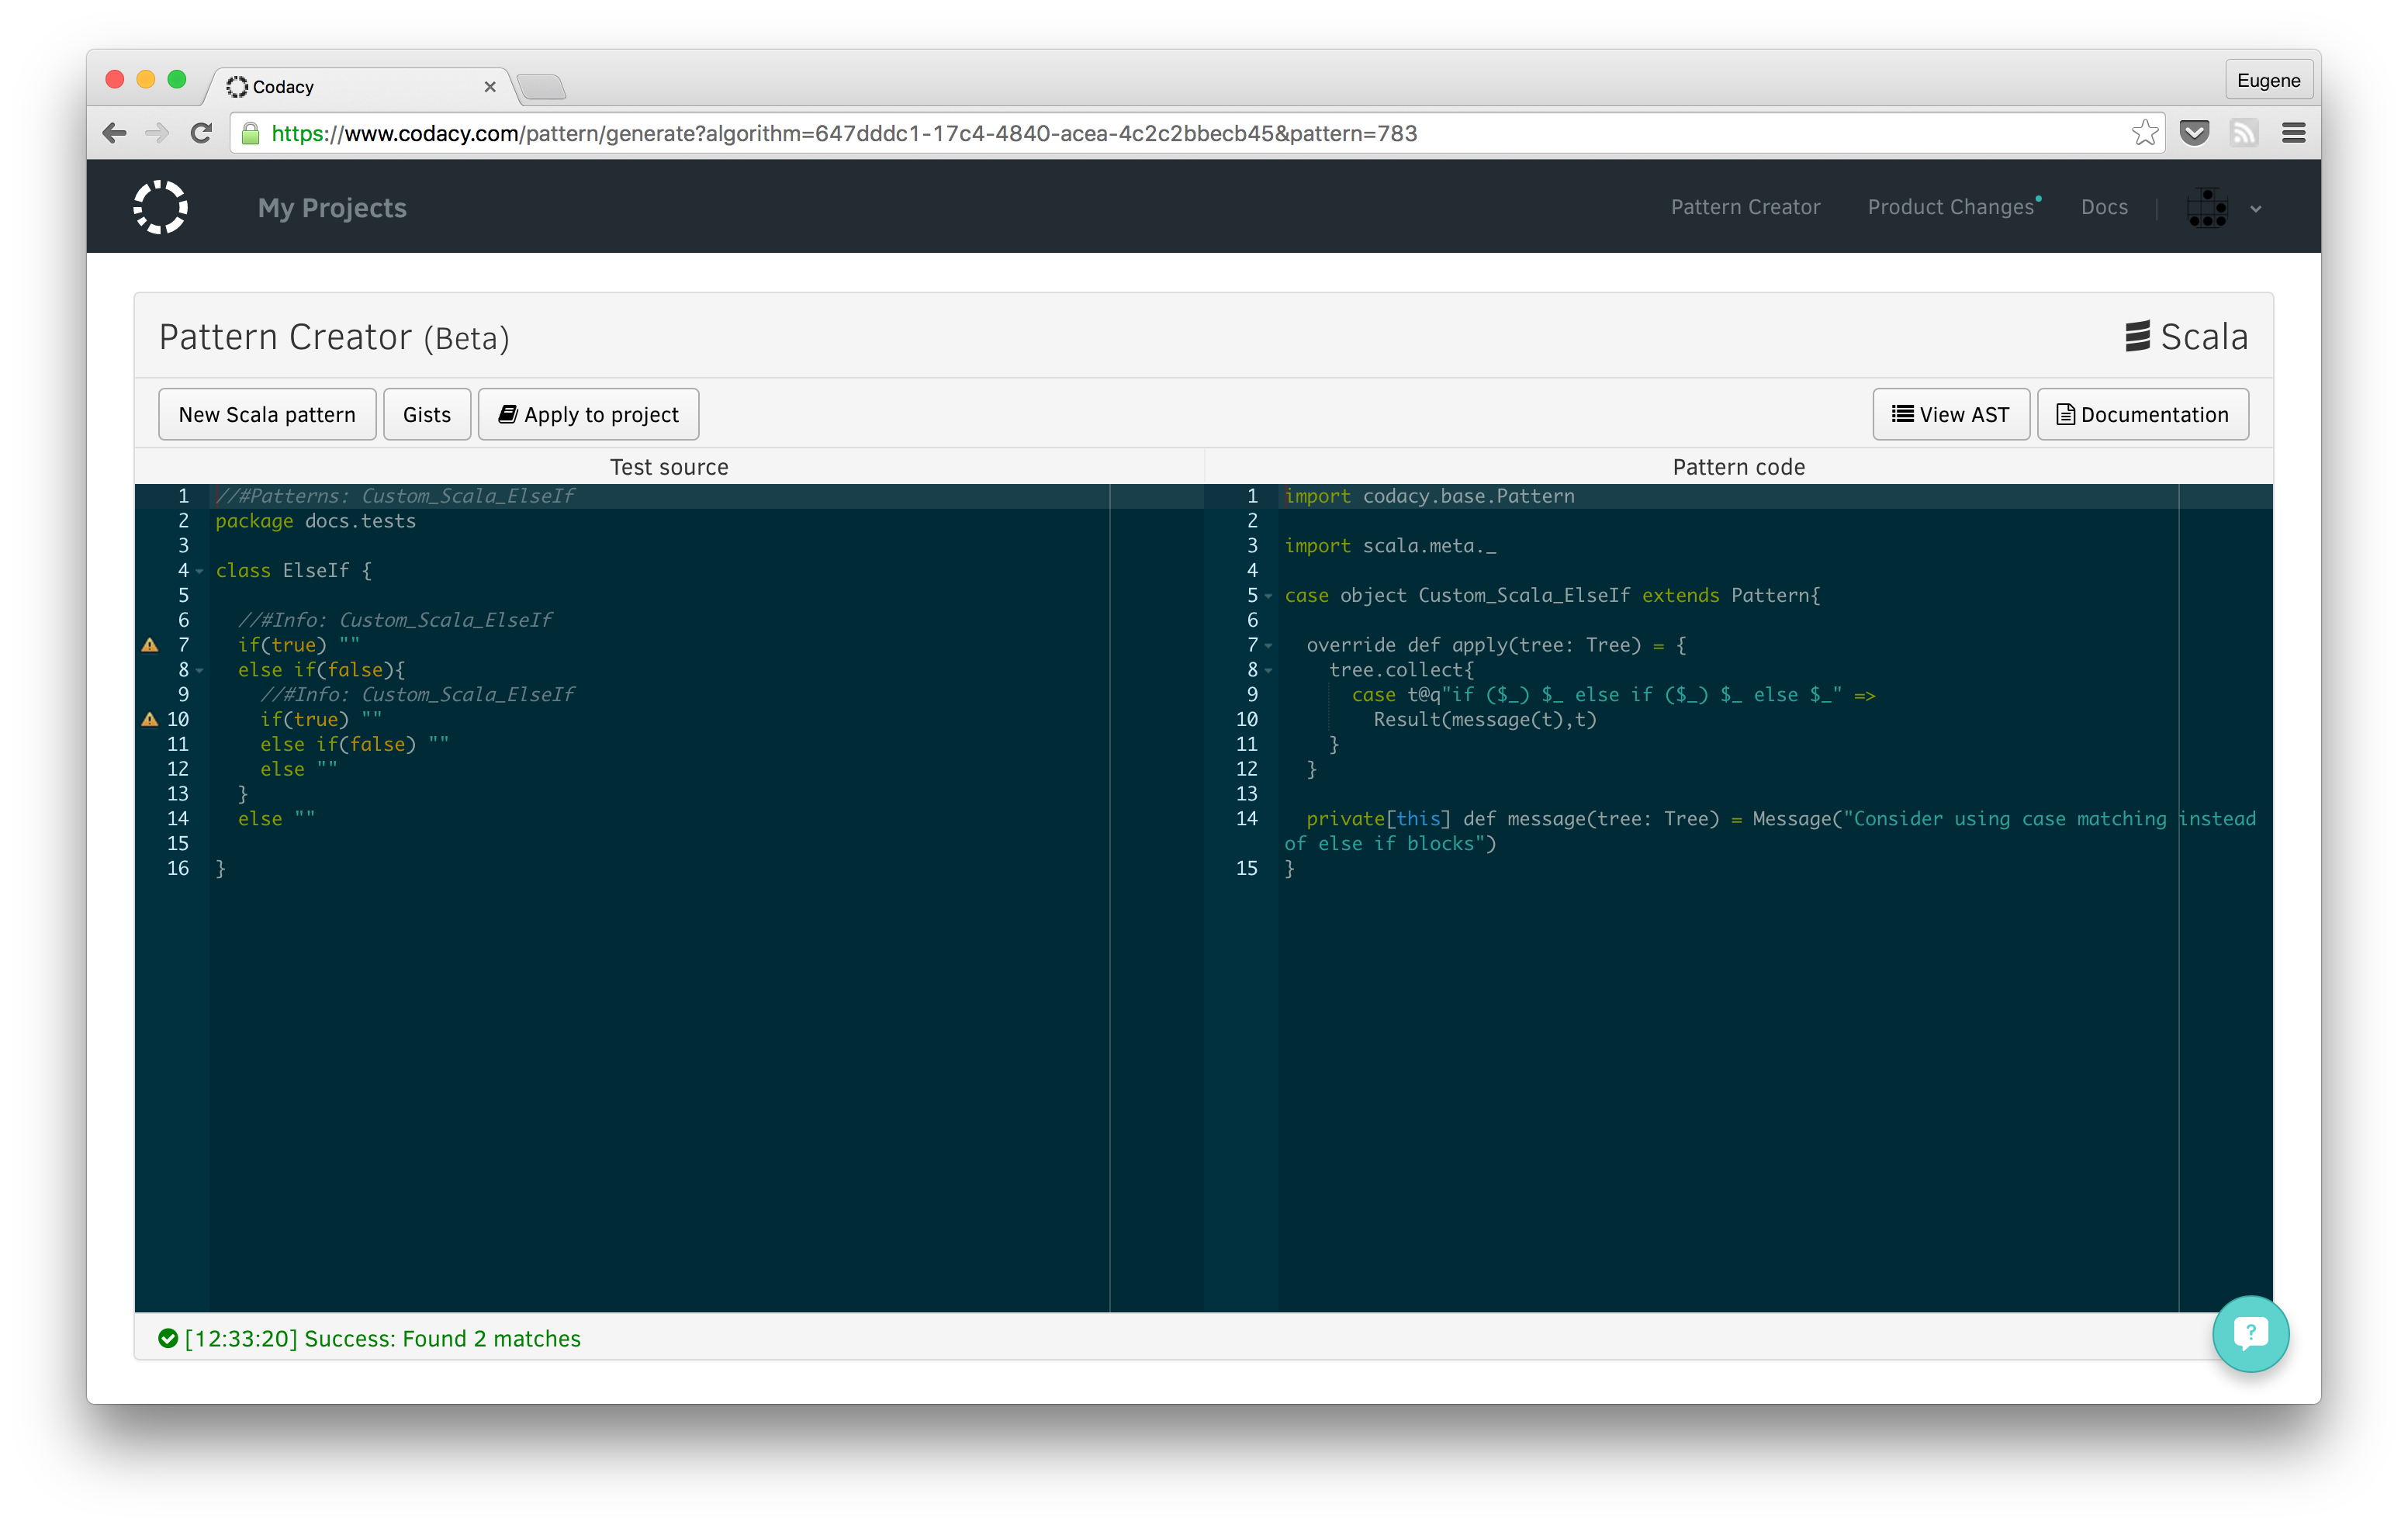
\includegraphics[height=7.5cm]{codacy.png}
\end{center}
\end{frame}

\begin{frame}{How Codacy's Scala engine works}
\begin{itemize}
\item Used to run on scala.reflect toolboxes
\item Now using a much more precise scala.meta's parser thanks to the joint work of Johann Egger and Mathieu Demarne
\item Code patterns are written with quasiquotes
\item More than 80 patterns implemented
\end{itemize}
\end{frame}

\begin{frame}{Future plans}
\begin{itemize}
\item More patterns, focused on security
\item Looking forward to scala.meta's semantic API
\end{itemize}
\end{frame}

\begin{frame}{Now open-source!}
\begin{itemize}
\item Most of the Scala patterns were open-sourced yesterday
\item Automatic deployment of pull requests is on its way
\item Check it out at \text{\color{blue}\href{https://github.com/codacy/codacy-scalameta}{https://github.com/codacy/codacy-scalameta}}
\end{itemize}
\end{frame}

\sectionframe{Case study: Scalafmt}

\begin{frame}[c, fragile]{Better things to do than argue about formatting}
\vskip20pt
\begin{center}
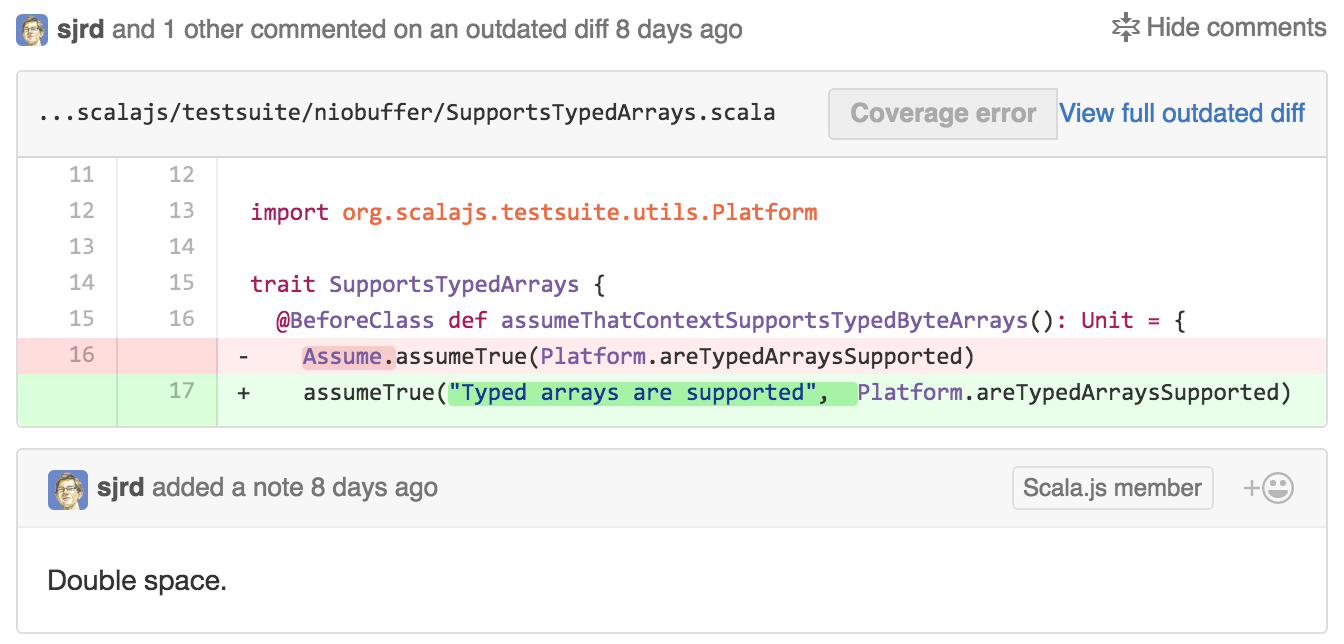
\includegraphics[width=0.9\linewidth]{time-sink.png}
\end{center}
\end{frame}

\begin{frame}[c, fragile]{Code formatting should be automated}
\vskip20pt
\begin{center}
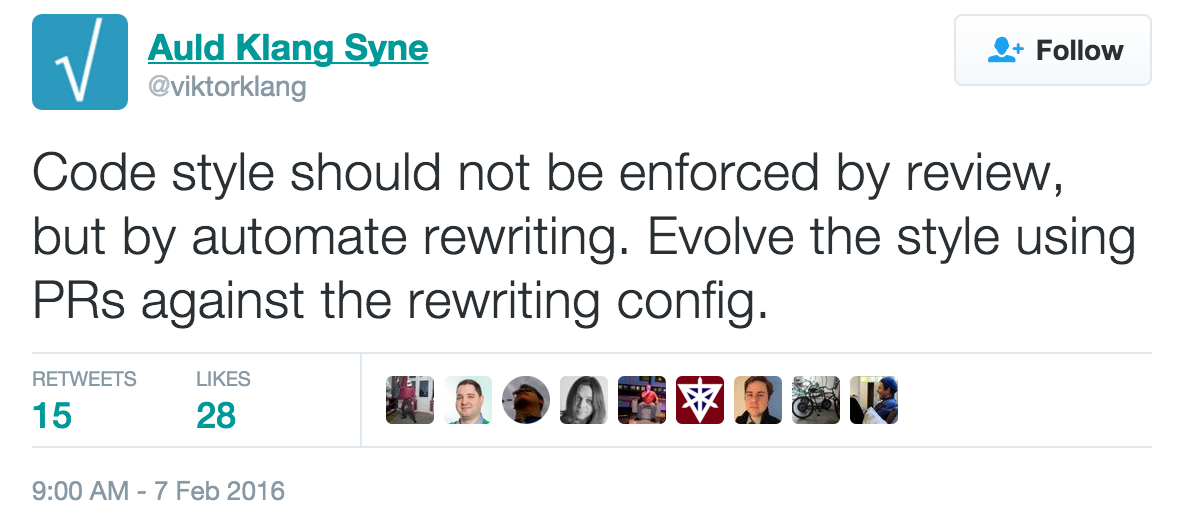
\includegraphics[width=0.9\linewidth]{klang.png}
\end{center}
\end{frame}

\begin{frame}[c, fragile]{Live demo!}
\vskip20pt
\begin{center}
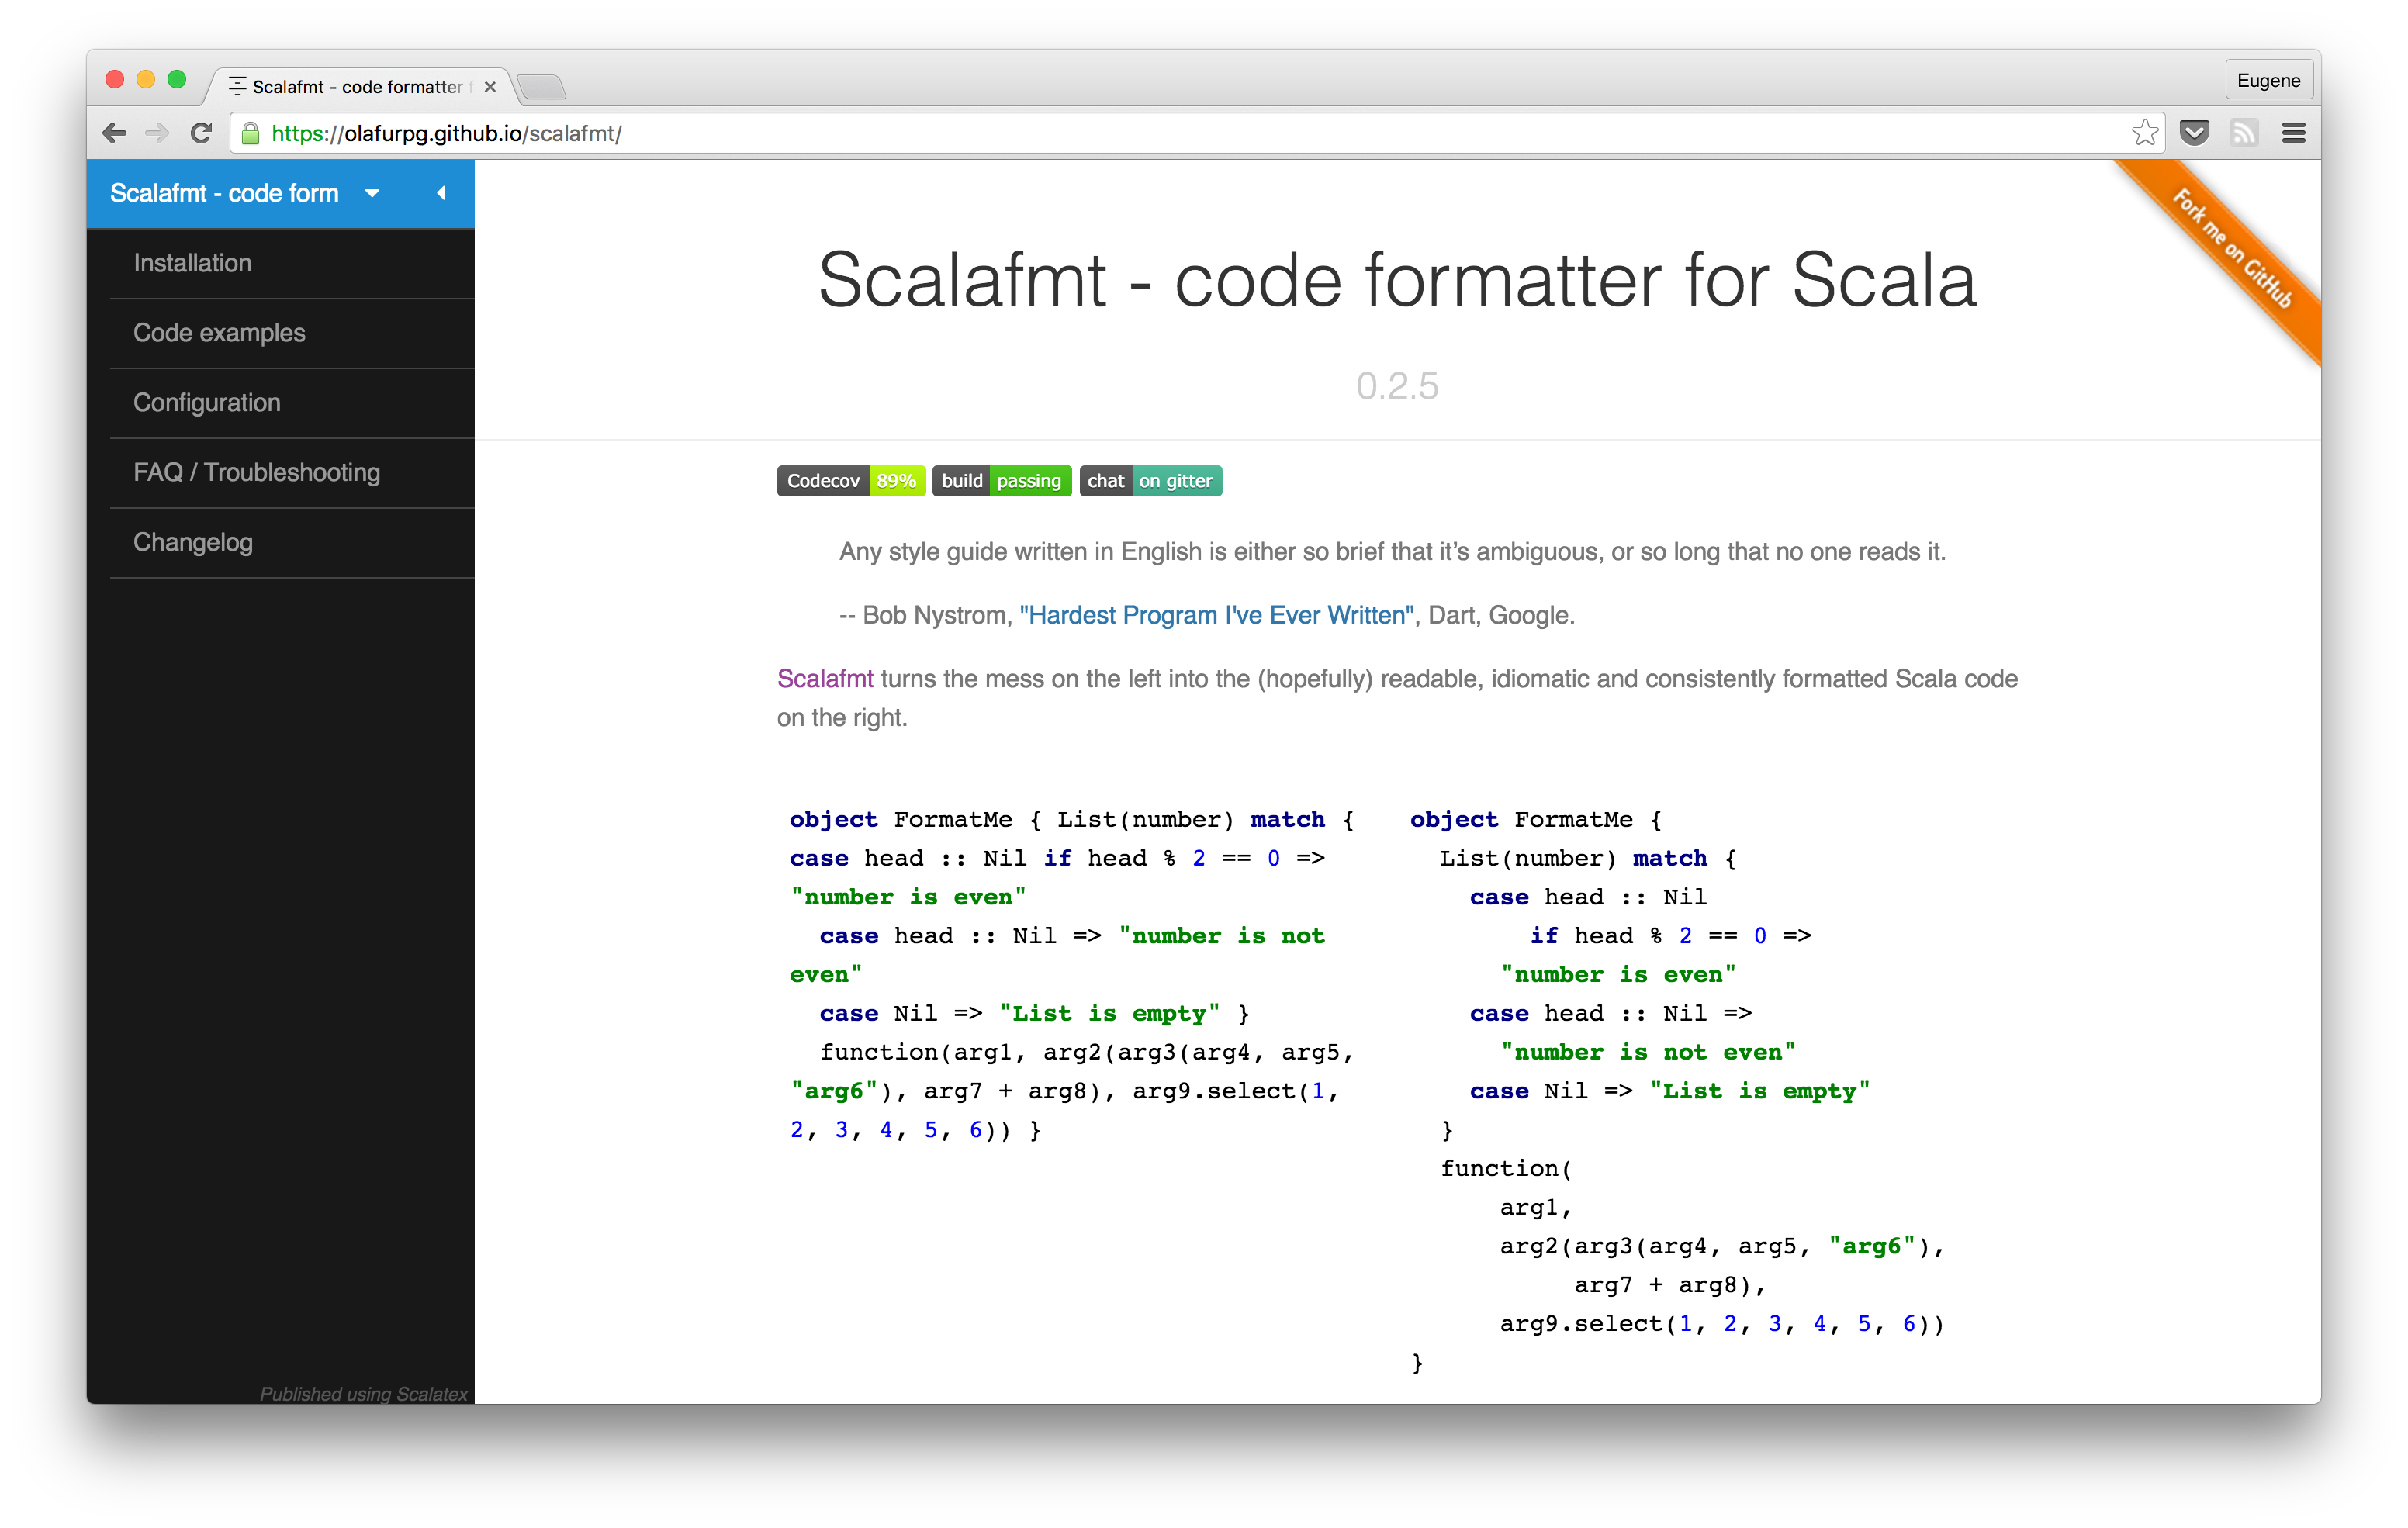
\includegraphics[width=0.9\linewidth]{scalafmt.png}
\end{center}
\end{frame}

\begin{frame}{How scalafmt works: example snippet}
\begin{semiverbatim}
class Point(x: Int, y: Int)
\end{semiverbatim}
\end{frame}

\begin{frame}[c, fragile]{How scalafmt works: unformatted tokens}
\vskip20pt
\begin{center}
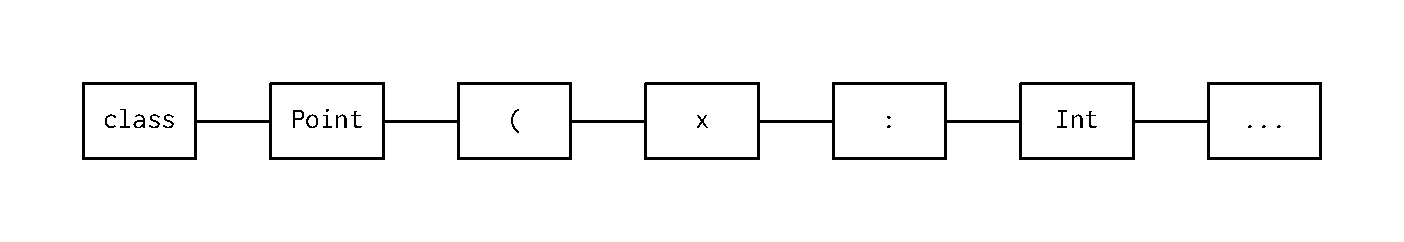
\includegraphics[width=0.9\linewidth]{tokens-raw.pdf}
\end{center}
\end{frame}

\begin{frame}[c, fragile]{How scalafmt works: formatted tokens}
\vskip20pt
\begin{center}
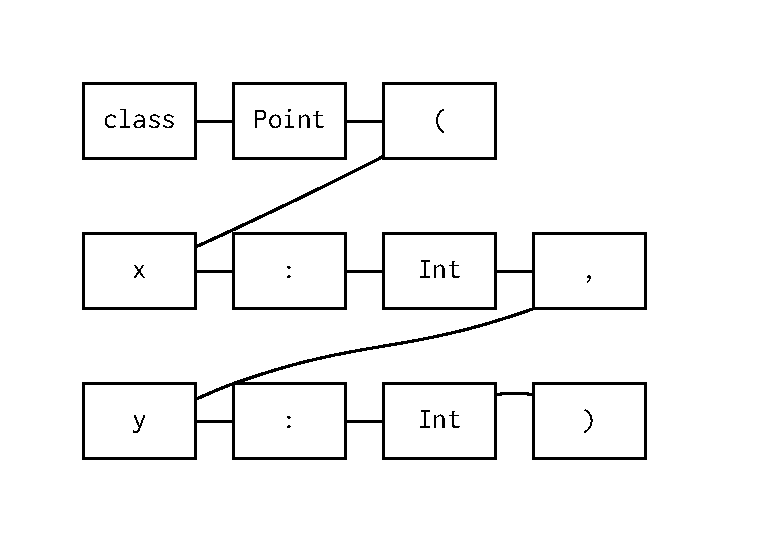
\includegraphics[width=0.9\linewidth]{tokens-formatted.pdf}
\end{center}
\end{frame}

\begin{frame}{Future plans}
\begin{itemize}
\item Out-of-the-box presets supporting popular code styles
\item Support for diff formatting
\item Performance improvements
\end{itemize}
\end{frame}

\sectionframe{Part 3: What will happen next?}

\begin{frame}{Graduation}
\begin{itemize}
\item It's been a fun five PhD years at EPFL
\item But it's time to wrap it up
\item Thesis defense incoming in 3... 2... 1...
\end{itemize}
\end{frame}

\begin{frame}{My next adventure}
\vskip20pt
\begin{center}

\includegraphics[height=4cm]{twitter.png}
\end{center}
\end{frame}

\begin{frame}{The arrangement with Twitter}
\begin{itemize}
\item 50\% of the time: working on my open-source Scala projects
\item 50\% of the time: making Scala tooling at Twitter better
\end{itemize}
\end{frame}

\begin{frame}{Next steps with scala.meta}
\begin{itemize}
\item Semantic API: typechecking, name resolution, implicit inference, etc
\item New-style (``inline'') macros
\item Other execution environments (2.10, 2.12, scala.js)
\end{itemize}
\end{frame}

\sectionframe{Summary}

\begin{frame}{Scala Macros}
\begin{itemize}
\item Macros are not going away
\item Will be replaced with a better version based on scala.meta
\item I'm graduating soon, but still going to be the project lead
\end{itemize}
\end{frame}

\begin{frame}{Scala Meta}
\begin{itemize}
\item The project is officially endorsed and funded
\item Just released v1.0
\item Jetbrains, Codacy and Scalafmt are already building cool stuff with it
\item Join us in our quest for next-generation tooling!
\end{itemize}
\end{frame}

\end{document}
